\section{Introduction}
\begin{frame}{}
    \LARGE GANs: \textbf{Introduction}
\end{frame}

\begin{frame}[allowframebreaks]{Comparing Distributions via Samples}
Given a finite set of samples from two distributions $S_1 = \{x \sim P\}$ and $S_2 = \{x \sim Q\}$, how can we tell if these samples are from the same distribution? (i.e., $P = Q$?)
\begin{figure}
    \centering
    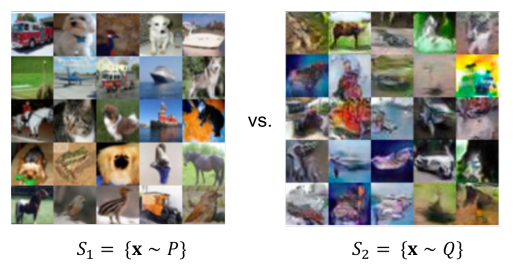
\includegraphics[height=0.58\textheight, width=\textwidth, keepaspectratio]{images/gan/gan_two_dist.png}
\end{figure}

% Place this at the bottom of the frame, before \end{frame}
% \vspace{0.5em}
\begin{minipage}{\textwidth}
\footnotetext{GANs aim to replicate data distributions, but we rarely have access to
the true probability distribution function. Instead, we compare samples
from the real data distribution with those generated by the model.}
\end{minipage}

\framebreak

\begin{itemize}
    \item Let's consider a test statistic $T$ for this purpose.
    \item Test statistic $T$ compares $S_1$ and $S_2$ e.g., difference in means, variances of the two sets of samples.
    \item \textbf{Key observation}: Test statistic is likelihood-free since it does not involve the densities $P$ or $Q$ (only samples)
\end{itemize}
\end{frame}